\section{Method}
\label{sec:method}

In the following, we introduce the mathematical formulation of the weakly-supervised 3D shape completion problem. Subsequently, we briefly discuss denoising variational auto-encoders (\DVAEs) \citep{Kingma2014ICLR,Im2017AAAI} which we use to learn a strong shape prior \red{that embeds a set of reference shapes in a low-dimensional latent space.} Then, we formally derive our proposed amortized maximum likelihood (\AML) approach. \red{Here, we use maximum likelihood to learn an embedding of the observations within the same latent space -- thereby allowing to perform shape completion.} The overall approach is also illustrated in \figref{fig:method}.

\subsection{Problem Formulation}
\label{subsec:method-problem}

\newcommand{\shapeneta}{330} % 726 297
\newcommand{\shapenetb}{66}
\newcommand{\shapenetc}{132}
\newcommand{\shapenetd}{198}
\newcommand{\shapenete}{726}

\begin{figure}
    \vspace*{-\figskipabove px}
    \centering
    
    \begin{subfigure}[t]{0.5\textwidth}
        \begin{subfigure}{0.19\textwidth}
            \centering\vspace{0px}
            \includegraphics[height=1.5cm,trim={\cropleft cm \croplower cm \cropright cm \cropupper cm},clip]{gdat_shapenet_clean_low_\shapeneta_gt_only}
        \end{subfigure}
        \begin{subfigure}{0.19\textwidth}
            \centering\vspace{0px}
            \includegraphics[height=1.5cm,trim={\cropleft cm \croplower cm \cropright cm \cropupper cm},clip]{gdat_shapenet_clean_low_\shapenetb_gt_only}
        \end{subfigure}
        \begin{subfigure}{0.19\textwidth}
            \centering\vspace{0px}\textbf{}
            \includegraphics[height=1.5cm,trim={\cropleft cm \croplower cm \cropright cm \cropupper cm},clip]{gdat_shapenet_clean_low_\shapenetc_gt_only}
        \end{subfigure}
        \begin{subfigure}{0.19\textwidth}
            \centering\vspace{0px}
            \includegraphics[height=1.5cm,trim={\cropleft cm \croplower cm \cropright cm \cropupper cm},clip]{gdat_shapenet_clean_low_\shapenetd_gt_only}
        \end{subfigure}
        \begin{subfigure}{0.19\textwidth}
            \centering\vspace{0px}
            \includegraphics[height=1.5cm,trim={\cropleft cm \croplower cm \cropright cm \cropupper cm},clip]{gdat_shapenet_clean_low_\shapenete_gt_only}
        \end{subfigure}
        \subcaption{Reference Shapes $\mathcal{Y}$}
    \end{subfigure}
    \\
    \begin{subfigure}[t]{0.29\textwidth}
        \begin{subfigure}[t]{0.49\textwidth}
            \centering\vspace{0px}
            \includegraphics[height=2cm,trim={\cropleft cm \croplower cm \cropright cm \cropupper cm},clip]{gdat_shapenet_clean_low_\shapeneta_bin_points}
        \end{subfigure}
        \begin{subfigure}[t]{0.49\textwidth}
            \centering\vspace{0px}
            \includegraphics[height=2cm,trim={\cropleft cm \croplower cm \cropright cm \cropupper cm},clip]{gdat_shapenet_clean_low_\shapeneta_bin_space}
        \end{subfigure}
        \subcaption{Observation $x_n$}
    \end{subfigure}
    \hfill
    \begin{subfigure}[t]{0.18\textwidth}
        \centering\vspace{0px}
        \includegraphics[height=2cm,trim={\cropleft cm \croplower cm \cropright cm \cropupper cm},clip]{gdat_shapenet_clean_low_\shapeneta_bin_only}
        \subcaption{Ground Truth $y_n^*$}
    \end{subfigure}
    \vspace*{-\figskipcaption px}
    \caption{{\bf Weakly-Supervised Shape Completion.} Given reference shapes $\mathcal{Y}$ and incomplete observations $\mathcal{X}$, we want to learn a mapping $x_n \mapsto \tilde{y}(x_n)$ such that $\tilde{y}(x_n)$ matches the \emph{unknown} ground truth shape $y_n^*$ as close as possible. The observations $x_n$ are split into free space (\ie, $x_{n,i} = 0$, right) and point observations (\ie, $x_{n,i} = 1$, left). Shapes are shown in {\color{rbeige}beige} and observations in {\color{rred}red}.}
    \label{fig:method-problem}
    \vspace*{-\figskipbelow px}
\end{figure}

In a supervised setting, the task of 3D shape completion can be described as follows: Given a set of incomplete observations $\mathcal{X} = \{x_n\}_{n = 1}^N \subseteq \mathbb{R}^R$ and corresponding ground truth shapes $\mathcal{Y}^* = \{y_n^*\}_{n = 1}^N \subseteq \mathbb{R}^R$, learn a mapping $x_n \mapsto y_n^*$ that is able to generalize to previously unseen observations and possibly across object categories. We assume $\mathbb{R}^R$ to be a suitable representation of observations and shapes; in practice, we resort to occupancy grids and signed distance functions (SDFs) defined on regular grids, \ie, $x_n, y_n^* \in \mathbb{R}^{H \ntimes W \ntimes D} \simeq \mathbb{R}^R$. Specifically, occupancy grids indicate occupied space, \ie, voxel $y_{n,i}^* = 1$ if and only if the voxel lies on or inside the shape's surface. To represent shapes with sub-voxel accuracy, SDFs hold the distance of each voxel's center to the surface; for voxels inside the shape's surface, we use negative sign.
Finally, for the (incomplete) observations, we write $x_n \in \{0, 1, \uk\}^R$ to make missing information explicit; in particular, $x_{n,i} = \uk$ corresponds to unobserved voxels, while $x_{n,i} = 1$ and $x_{n,i} = 0$ correspond to occupied and unoccupied voxels, respectively.

On real data, \eg, KITTI \citep{Geiger2012CVPR}, supervised learning is often not possible as obtaining ground truth annotations is labor intensive, \cf \citep{Menze2015CVPR,Xie2016CVPR}. Therefore, we target a weakly-supervised variant of the problem instead: Given observations $\mathcal{X}$ and reference shapes $\mathcal{Y} = \{y_m\}_{m = 1}^M \subseteq \mathbb{R}^R$ both of the same, known object category, learn a mapping $x_n \mapsto \tilde{y}(x_n)$ such that the predicted shape $\tilde{y}(x_n)$ matches the unknown ground truth shape $y_n^*$ as close as possible -- or, in practice, the sparse observation $x_n$ while being plausible considering the set of reference shapes, \cf \figref{fig:method-problem}. Here, supervision is provided in the form of the known object category. Alternatively, the reference shapes $\mathcal{Y}$ can also include multiple object categories resulting in an even weaker notion of supervision as the correspondence between observations and object categories is unknown. \red{Except for the object categories, however, the set of reference shapes $\mathcal{Y}$, and its size $M$, is completely independent of the set of observations $\mathcal{X}$, and its size $N$, as also highlighted in \figref{fig:method}.} On real data, \eg, KITTI, we additionally assume the object locations to be given in the form of 3D bounding boxes in order to extract the corresponding observations $\mathcal{X}$. In practice, the reference shapes $\mathcal{Y}$ are derived from watertight, triangular meshes, \eg, from ShapeNet \citep{Chang2015ARXIV} or ModelNet \citep{Wu2015CVPR}.

\subsection{Shape Prior}
\label{subsec:method-prior}

\red{We approach the weakly-supervised shape completion problem by first learning a shape prior using a denoising variational auto-encoder (\DVAE). Later, this prior constrains shape inference (see \secref{subsec:method-inference}) to predict reasonable shapes. In the following, we briefly discuss the standard variational auto-encoder (\VAE), as introduced by \cite{Kingma2014ICLR}, as well as its denoising extension, as proposed by \cite{Im2017AAAI}.}

\boldparagraph{Variational Auto-Encoder (\VAE)}
%
We propose to use the provided reference shapes $\mathcal{Y}$ to learn a \red{generative} model of possible 3D shapes over a low-dimensional latent space $\mathcal{Z} = \mathbb{R}^Q$, \ie,  $Q \ll R$. \red{In the framework of \VAEs, the joint distribution $p(y, z)$ of shapes $y$ and latent codes $z$} decomposes into $p(y | z)p(z)$ with $p(z)$ being a unit Gaussian, \ie, $\mathcal{N}(z;0, I_Q)$ and $I_Q \in \mathbb{R}^{R \times R}$ being the identity matrix. \red{This decomposition allows to sample $z \sim p(z)$ and $y \sim p(y|z)$ to generate random shapes.}
\red{For training, however, we additionally need to approximate the posterior $p(z | y)$.} \red{To this end, the so-called recognition model $q(z | y) \approx p(z | y)$} takes the form
%
\begin{align}
q(z | y) &= \mathcal{N}(z; \mu(y), \text{diag}(\sigma^2(y)))\label{eq:encoder-decoder}
\end{align}
%
where $\mu(y), \sigma^2(y) \in \mathbb{R}^Q$ are predicted using the encoder neural network. \red{The generative model $p(y|z)$ decomposes over voxels $y_i$; the corresponding probabilities $p(y_i | z)$ are represented using Bernoulli distributions for occupancy grids or Gaussian distributions for SDFs:}
%
\begin{align}
    \begin{split}
        p(y_i | z) &= \text{Ber}(y_i ; \theta_i(z))\quad\text{or}\\
        p(y_i | z) &= \mathcal{N}(y_i ; \mu_i(z), \sigma^2).\label{eq:decoder}
    \end{split}
\end{align}
%
In both cases, the parameters, \ie, $\theta_i(z)$ or $\mu_i(z)$, are predicted using the decoder neural network. \red{For SDFs, we explicitly set $\sigma^2$ to be constant (see \secref{sec:training}). Then, $\sigma^2$ merely scales the corresponding loss, thereby implicitly defining the importance of accurate SDFs relative to occupancy grids as described below.}

In the framework of variational inference, the parameters of the encoder and the decoder \red{neural networks} are found by maximizing the likelihood $p(y)$. \red{In practice, the likelihood is usually intractable and the evidence lower bound is maximized instead, see \citep{Kingma2014ICLR,Blei2016ARXIV}. This results in the following loss to be minimized:}
%
\begin{align}
\mathcal{L}_{\text{VAE}}(w) = - \mathbb{E}_{q(z |y)}[\ln p(y|z)] + \text{KL}(q(z | y)| p(z)).\label{eq:vae}
\end{align}
%
\red{Here,} $w$ are the weights of the encoder and decoder \red{hidden in the recognition model $q(z | y)$ and the generative model $p(y | z)$, respectively}. \red{The Kullback-Leibler divergence $\text{KL}$ can be computed analytically as described in the appendix of \citep{Kingma2014ICLR}.} The negative log-likelihood $-\ln p(y|z)$ corresponds to a binary cross-entropy error for occupancy grids \red{and} a scaled sum-of-squared error for SDFs. The loss $\mathcal{L}_{\text{VAE}}$ is minimized using stochastic gradient descent (SGD) by approximating the expectation \red{using samples}:
%
\begin{align}
- \mathbb{E}_{q(z |y)}[\ln p(y|z)] \approx - \sum_{l = 1}^L \ln p(y | z^{(l)})
\end{align}
%
\red{The required samples $z^{(l)} \sim q(z|y)$ are computed using the so-called reparameterization trick,
\begin{align}
z^{(l)} = \mu(y) + \epsilon^{(l)} \sigma(y)\quad\text{with}\quad\epsilon^{(l)} \sim \mathcal{N}(\epsilon; 0, I_Q),\label{eq:repa}
\end{align}
in order to make $\mathcal{L}_{\text{VAE}}$, specifically the sampling process, differentiable.} \red{In practice, we found $L = 1$ samples to be sufficient -- which conforms with results by \cite{Kingma2014ICLR}. At test time, the sampling process $z\sim q(z|y)$ is replaced by the predicted mean $\mu(y)$.}
\red{Overall, the standard VAE allows us to embed the reference shapes in a low-dimensional latent space. In practice, however, the learned prior might still include unreasonable shapes.}

\boldparagraph{Denoising \VAE (\DVAE)}
%
\red{In order to avoid inappropriate shapes to be included in our shape prior, we consider a denoising variant of the \VAE allowing to obtain a tighter bound on the likelihood $p(y)$.} More specifically, a corruption process $y' \sim p(y' | y)$ is considered and the corresponding evidence lower bound results in the following loss:
%
\begin{align}
    \begin{split}
        \mathcal{L}_{\text{DVAE}}(w) = &- \mathbb{E}_{q(z | y')}[\ln p(y|z)]\\
        &+ \text{KL}(q(z | y')| p(z)).
    \end{split}
\end{align}
%
\red{Note that the reconstruction error $-\ln p(y|z)$ is still computed with respect to the uncorrupted shape $y$ while $z$, in contrast to \eqnref{eq:vae}, is sampled conditioned on the corrupted shape $y'$.} In practice, the corruption process $p(y' | y)$ is modeled using Bernoulli noise for occupancy grids and Gaussian noise for SDFs.
In experiments, we found \DVAEs to learn more robust latent spaces \red{-- meaning the prior is less likely to contain unreasonable shapes. In the following, we always use \DVAEs as shape priors.}

\subsection{Shape Inference}
\label{subsec:method-inference}

After learning the shape prior, \red{defining the joint distribution $p(y, z)$ of shapes $y$ and latent codes $z$ as product of generative model $p(y|z)$ and prior $p(z)$}, shape completion can be formulated as a maximum likelihood (\ML) problem \red{for $p(y, z)$} over the lower-dimensional latent space $\mathcal{Z} = \mathbb{R}^Q$. The corresponding negative log-likelihood $-\ln p(y, z)$ to be minimized can be written as
%
\begin{align}
\mathcal{L}_{\text{ML}}(z) &= - \sum_{x_i \neq \uk} \ln p(y_i = x_i | z) - \ln p(z).\label{eq:ml}
\end{align}
%
As the prior $p(z)$ is Gaussian, the negative log-probability $- \ln p(z)$ is proportional to $\|z\|_2^2$ and \red{constrains the problem to likely, \ie, reasonable, shapes with respect to the shape prior}. As before, the generative model $p(y | z)$ decomposes over voxels; here, we can only consider actually observed voxels $x_i \neq \uk$. \red{We assume that the learned shape prior can complete the remaining, unobserved voxels $x_i = \uk$.} Instead of solving \eqnref{eq:ml} for each observation $x \in \mathcal{X}$ independently, however, we follow the idea of amortized inference \citep{Gersham2014COGSCI} and train a \red{new} encoder $z(x;w)$ to \emph{learn} \ML. To this end, we keep the generative model $p(y|z)$ fixed and train \red{only} the weights $w$ of the \red{new} encoder $z(x;w)$ using the \ML objective as loss:
%
\begin{align}
    \begin{split}
        \mathcal{L}_{\text{dAML}}(w) =& - \sum _{x_i \neq \uk} \ln p(y_i = x_i | z(x; w))\\
        &- \lambda \ln p(z(x; w)).\label{eq:aml}
    \end{split}
\end{align}
%
\red{Here,} $\lambda$ controls the importance of the shape prior. The exact form of the probabilities $p(y_i = x_i | z)$ depends on the used shape representation. For occupancy grids, this term results in a cross-entropy error as \red{both the predicted voxels $y_i$ and the observations $x_i$} are, for $x_i \neq \uk$, binary. For SDFs, however, the term is not well-defined as $p(y_i | z)$ is modeled with a continuous Gaussian distribution, while the observations $x_i$ are binary. As solution, we could compute (signed) distance values along the rays corresponding to observed points (\eg, following \citep{Steinbrucker2013ICCV}) in order to obtain continuous observations $x_i \in\mathbb{R}$ for $x_i \neq \uk$. However, as illustrated in \figref{fig:method-sdf}, noisy observations cause the distance values along the whole ray to be invalid. This can partly be avoided when relying \red{only} on occupancy to represent the observations; in this case, free space (\cf \figref{fig:method-problem}) observations are partly correct even though observed points may lie within the corresponding shapes.

For making SDFs tractable (\ie, to predict sub-voxel accurate, visually smooth and appealing shapes, see \secref{sec:experiments}) \red{while using binary observations}, we propose to define $p(y_i = x_i | z)$ through a simple transformation. In particular, as $p(y_i | z)$ is modeled using a Gaussian distribution $\mathcal{N}(y_i ; \mu_i(z), \sigma^2)$ where $\mu_i(z)$ is predicted using the fixed decoder ($\sigma^2$ is constant), and $x_i$ is binary (for $x_i \neq \uk$), we introduce a mapping $\theta_i(\mu_i(z))$ transforming the predicted \red{mean SDF value to an occupancy probability} $\theta_i(\mu_i(z))$:
%
\begin{align}
p(y_i = x_i | z) = \text{Ber}(y_i = x_i; \theta_i(\mu_i(z)))
\end{align}
%
As, \red{by construction (see \secref{subsec:method-problem}), occupied voxels have negative sign or value zero in the SDF}, we can derive the occupancy probability $\theta_i(\mu_i(z))$ as the probability of a non-positive distance:
%
\begin{align}
\theta_i(\mu_i(z)) &= \mathcal{N}(y_i \leq 0; \mu_i(z), \sigma^2)\\[3px]
&= \frac{1}{2} \left(1 + \text{erf}\left(\frac{- \mu_i(z)}{\sigma \sqrt{\pi}}\right)\right).\label{eq:sdf}
\end{align}
%
Here, $\text{erf}$ is the error function which, in practice, can be approximated following~\citep{Abramowitz1974}. \eqnref{eq:sdf} is illustrated in \figref{fig:method-sdf} where the occupancy probability $\theta_i(\mu_i(z))$ is computed as the area under the Gaussian bell curve for $y_i \leq 0$. This per-voxel transformation can easily be implemented as non-linear layer and its derivative \wrt $\mu_i(z)$
is, by construction, a Gaussian. \red{Note that the transformation is correct, not approximate, based on our model assumptions and the definitions in \secref{subsec:method-problem}.} \red{Overall, this transformation allows us to easily minimize \eqnref{eq:aml} for both occupancy grids and SDFs using binary observations. The obtained encoder embeds the observations in the latent shape space to perform shape completion.}

\begin{figure}[t]
	\vspace*{-\figskipabove px}
	\centering
	\hfill
	\begin{subfigure}[t]{0.25\linewidth}
		\vspace{0px}
		\centering
		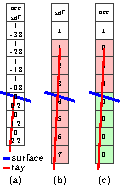
\includegraphics[height=4.5cm]{fig_method_sdf_2}
	\end{subfigure}
	\begin{subfigure}[t]{0.6\linewidth}
		\vspace{3px}
		\centering
		\hspace*{-12px}
		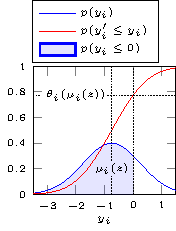
\includegraphics[height=4.5cm]{fig_method_sdf_1}
	\end{subfigure}
	\hfill
	\vspace*{-8px}
	\caption{{{\bf Left: Problem with SDF Observations.} Illustration of a ray ({\color{red}red line}) correctly hitting a surface ({\color{blue}blue line}) causing the (signed) distance values and occupancy values computed for voxels along the ray to be correct (\cf (a)). A noisy ray, however, causes all voxels along the ray to be assigned incorrect distance values (marked {\colorbox{red!25}{red}}) \wrt to the true surface ({\color{blue}blue line}) because the ray ends far behind the actual surface (\cf (b)). When using occupancy only, in contrast, only the voxels behind the surface are assigned invalid occupancy states (marked {\colorbox{red!25}{red}}); the remaining voxels are labeled correctly (marked {\colorbox{green!25}{green}}; \cf (c)).
			{\bf Right: Proposed Gaussian-to-Bernoulli Transformation.} For $p(y_i) := p(y_i | z) = \mathcal{N}(y_i;\mu_i(z), \sigma^2)$ ({\color{blue}blue}), we illustrate the transformation discussed in \secref{subsec:method-inference} allowing to use the binary observations $x_i$ (for $x_i \neq \uk$) to supervise the SDF predictions. This is achieved by transforming the predicted Gaussian distribution to a Bernoulli distribution with occupancy probability $\theta_i(\mu_i(z)) = p(y_i \leq 0)$ ({\color{blue}blue area}).}}
	\label{fig:method-sdf}
	\vspace*{-\figskipbelow px}
\end{figure}

\subsection{Practical Considerations}

\begin{figure*}[ht]
    \vspace*{-\figskipabove px}
    \vspace*{2px}
	\centering
        
	\begin{subfigure}[t]{0.32\textwidth}
        \centering\vspace{0px}
   		\begin{subfigure}[t]{0.32\textwidth}
   			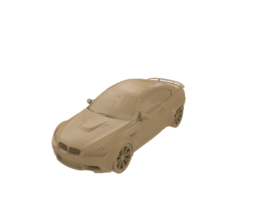
\includegraphics[width=1.75cm,trim={\cropleft cm \croplower cm \cropright cm \cropupper cm},clip]{gdat_shapenet_clean_low_0_ori}
   		\end{subfigure}
   		\begin{subfigure}[t]{0.32\textwidth}
   			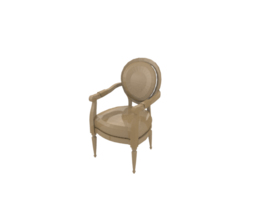
\includegraphics[width=1.75cm,trim={\cropleft cm \croplower cm \cropright cm \cropupper cm},clip]{gdat_modelnet_chair_low_1188_ori}
   		\end{subfigure}
   		\begin{subfigure}[t]{0.32\textwidth}
   			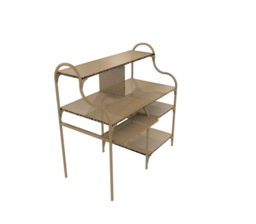
\includegraphics[width=1.75cm,trim={\cropleft cm \croplower cm \cropright cm \cropupper cm},clip]{gdat_modelnet_desk_low_0_ori}
   		\end{subfigure}
        \subcaption{Original}
		\label{fig:data-shapenet-modelnet-a}
	\end{subfigure}
	\begin{subfigure}[t]{0.32\textwidth}
        \centering\vspace{0px}
   		\begin{subfigure}[t]{0.32\textwidth}
   			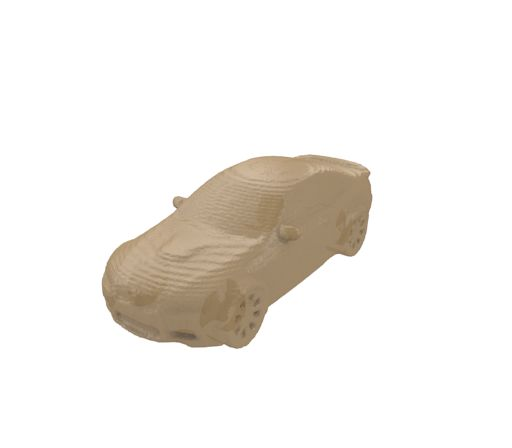
\includegraphics[width=1.75cm,trim={\cropleft cm \croplower cm \cropright cm \cropupper cm},clip]{gdat_shapenet_clean_low_0_wt}
   		\end{subfigure}
   		\begin{subfigure}[t]{0.32\textwidth}
   			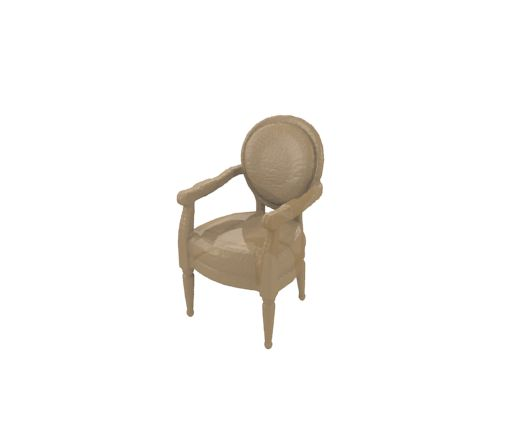
\includegraphics[width=1.75cm,trim={\cropleft cm \croplower cm \cropright cm \cropupper cm},clip]{gdat_modelnet_chair_low_1188_wt}
   		\end{subfigure}
   		\begin{subfigure}[t]{0.32\textwidth}
   			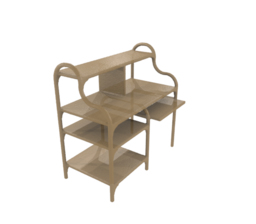
\includegraphics[width=1.75cm,trim={\cropleft cm \croplower cm \cropright cm \cropupper cm},clip]{gdat_modelnet_desk_low_0_wt}
   		\end{subfigure}
        \subcaption{TSDF Fusion, $256^3$}
		\label{fig:data-shapenet-modelnet-b}
	\end{subfigure}
	\begin{subfigure}[t]{0.32\textwidth}
		\centering\vspace{0px}
   		\begin{subfigure}[t]{0.32\textwidth}
   			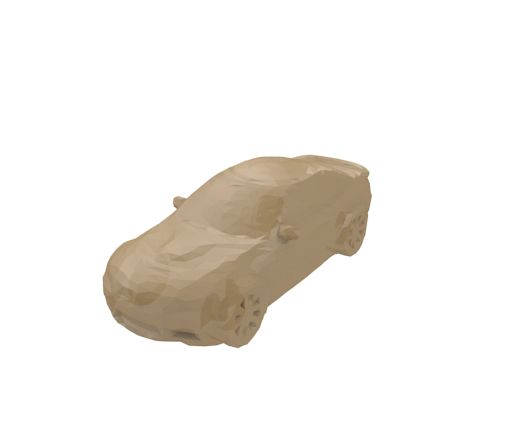
\includegraphics[width=1.75cm,trim={\cropleft cm \croplower cm \cropright cm \cropupper cm},clip]{gdat_shapenet_clean_low_0_simp}
   		\end{subfigure}
   		\begin{subfigure}[t]{0.32\textwidth}
   			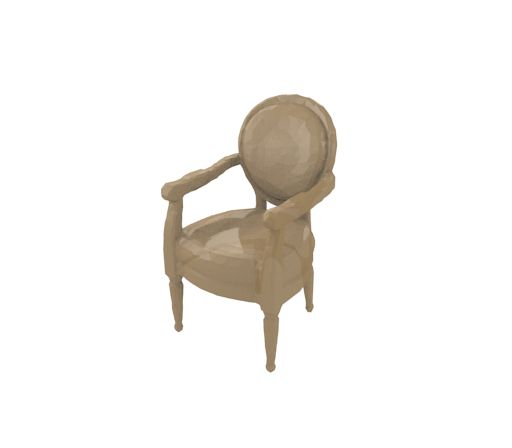
\includegraphics[width=1.75cm,trim={\cropleft cm \croplower cm \cropright cm \cropupper cm},clip]{gdat_modelnet_chair_low_1188_simp}
   		\end{subfigure}
   		\begin{subfigure}[t]{0.32\textwidth}
   			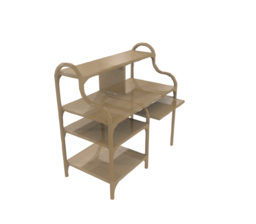
\includegraphics[width=1.75cm,trim={\cropleft cm \croplower cm \cropright cm \cropupper cm},clip]{gdat_modelnet_desk_low_0_simp}
   		\end{subfigure}
        \subcaption{Simplification, $5\text{k}$ Faces}
		\label{fig:data-shapenet-modelnet-c}
	\end{subfigure}
	\\
	\begin{subfigure}[t]{0.32\textwidth}
        \centering\vspace{0px}
   		\begin{subfigure}[t]{0.32\textwidth}
   			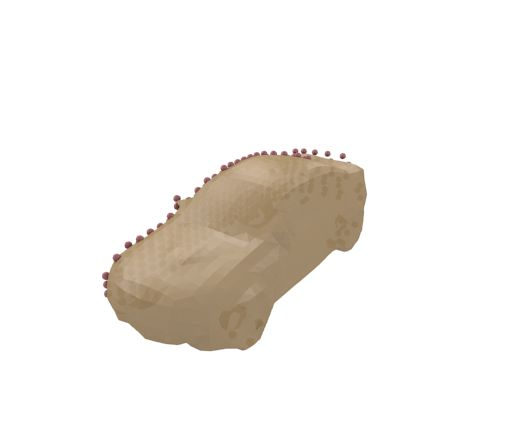
\includegraphics[width=1.75cm,trim={\cropleft cm \croplower cm \cropright cm \cropupper cm},clip]{gdat_shapenet_clean_low_0_rec}
   		\end{subfigure}
   		\begin{subfigure}[t]{0.32\textwidth}
   			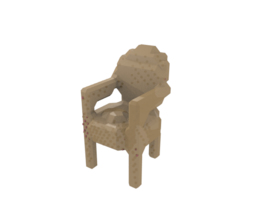
\includegraphics[width=1.75cm,trim={\cropleft cm \croplower cm \cropright cm \cropupper cm},clip]{gdat_modelnet_chair_low_1188_rec}
   		\end{subfigure}
   		\begin{subfigure}[t]{0.32\textwidth}
   			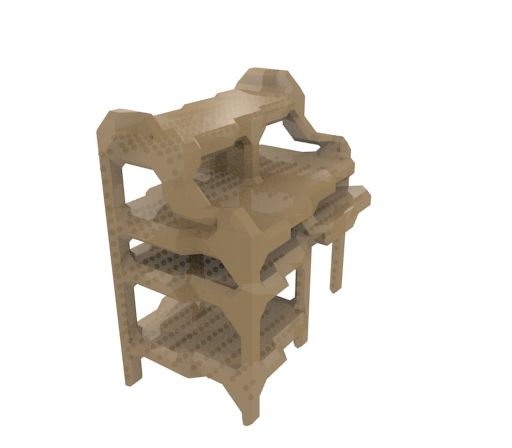
\includegraphics[width=1.75cm,trim={\cropleft cm \croplower cm \cropright cm \cropupper cm},clip]{gdat_modelnet_desk_low_0_rec}
   		\end{subfigure}
        \subcaption{Reconstruction, $24\ntimes54\ntimes24$/$32^3$}
		\label{fig:data-shapenet-modelnet-d}
	\end{subfigure}
	\begin{subfigure}[t]{0.32\textwidth}
        \centering\vspace{0px}
   		\begin{subfigure}[t]{0.32\textwidth}
   			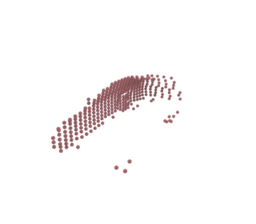
\includegraphics[width=1.75cm,trim={\cropleft cm \croplower cm \cropright cm \cropupper cm},clip]{gdat_shapenet_clean_low_0_points}
   		\end{subfigure}
   		\begin{subfigure}[t]{0.32\textwidth}
   			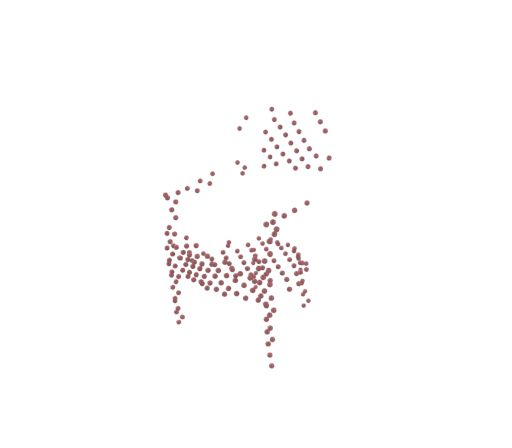
\includegraphics[width=1.75cm,trim={\cropleft cm \croplower cm \cropright cm \cropupper cm},clip]{gdat_modelnet_chair_low_1188_points}
   		\end{subfigure}
   		\begin{subfigure}[t]{0.32\textwidth}
   			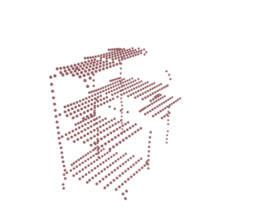
\includegraphics[width=1.75cm,trim={\cropleft cm \croplower cm \cropright cm \cropupper cm},clip]{gdat_modelnet_desk_low_0_points}
   		\end{subfigure}
        \subcaption{Observations}
		\label{fig:data-shapenet-modelnet-e}
	\end{subfigure}
	\begin{subfigure}[t]{0.32\textwidth}
        \centering\vspace{0px}
   		\begin{subfigure}[t]{0.32\textwidth}
   			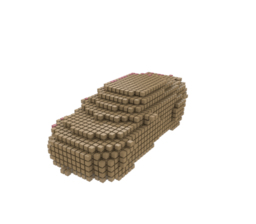
\includegraphics[width=1.75cm,trim={\cropleft cm \croplower cm \cropright cm \cropupper cm},clip]{gdat_shapenet_clean_low_0_bin}
   		\end{subfigure}
   		\begin{subfigure}[t]{0.32\textwidth}
   			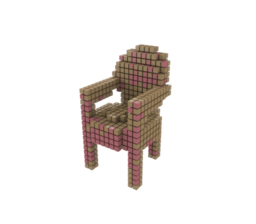
\includegraphics[width=1.75cm,trim={\cropleft cm \croplower cm \cropright cm \cropupper cm},clip]{gdat_modelnet_chair_low_1188_bin}
   		\end{subfigure}
   		\begin{subfigure}[t]{0.32\textwidth}
   			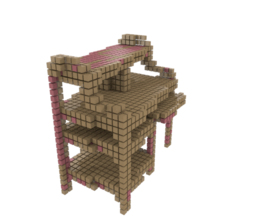
\includegraphics[width=1.75cm,trim={\cropleft cm \croplower cm \cropright cm \cropupper cm},clip]{gdat_modelnet_desk_low_0_bin}
   		\end{subfigure}
        \subcaption{Voxelization, $24\ntimes54\ntimes24$/$32^3$}
		\label{fig:data-shapenet-modelnet-f}
	\end{subfigure}
    \vspace*{-\figskipcaption px}
	\caption{{\bf ShapeNet and ModelNet Data Generation Pipeline.} On ShapeNet and ModelNet we illustrate: {\bf (\subref{fig:data-shapenet-modelnet-a})} samples from the original datasets; {\bf (\subref{fig:data-shapenet-modelnet-b})} fused watertight meshes from TSDF fusion at $256^3$ voxels resolution using \citep{Riegler2017THREEDV}; {\bf (\subref{fig:data-shapenet-modelnet-c})} simplified meshes ($5k$ faces); {\bf (\subref{fig:data-shapenet-modelnet-d})} marching cubes \citep{Lorensen1987SIGGRAPH} reconstructions from the SDFs computed from (\subref{fig:data-shapenet-modelnet-c}) (resolutions $24 \ntimes 54 \ntimes 24$ and $32^3$ voxels; note that steps (\subref{fig:data-shapenet-modelnet-b}) and (\subref{fig:data-shapenet-modelnet-c}) are necessary to derive exact SDFs); {\bf (\subref{fig:data-shapenet-modelnet-e})} observations obtained by projection into a single view; and {\bf (\subref{fig:data-shapenet-modelnet-f})} voxelized observations and shapes. Shapes (meshes and occupancy grids) {in \color{rbeige}beige} and observations in {\color{rred}red}.}
	\label{fig:data-shapenet-modelnet}
    \vspace*{-\figskipbelow px}
\end{figure*}

\boldparagraph{Encouraging Variety}
%
So far, our \AML formulation assumes a deterministic encoder $z(x,w)$ which predicts, given the observation $x$, a single code $z$ corresponding to a completed shape. A closer look at \eqnref{eq:aml}, however, reveals an unwanted problem: the data term scales with the number of observations, \ie, $|\{x_i \neq \uk\}|$, while the regularization term stays constant -- with less observations, the regularizer gains in importance leading to limited variety in the predicted shapes because $z(x; w)$ tends towards zero.

In order to encourage variety, we draw inspiration from the \VAE shape prior. Specifically, we use a probabilistic recognition model
%
\begin{align}
q(z|x) = \mathcal{N}(z; \mu(x), \text{diag}(\sigma^2(x)))
\end{align}
%
(\cf see \eqnref{eq:encoder-decoder}) and replace the negative log-likelihood $-\ln p(z)$ with the corresponding Kullback-Leibler divergence $\text{KL}(q(z|x)|p(z))$ with $p(z) = \mathcal{N}(z; 0, I_Q)$. Intuitively, this makes sure that the encoder's predictions ``cover'' the prior distribution -- thereby enforcing variety. Mathematically, the resulting loss, \ie, 
%
\begin{align}
\begin{split}
    \mathcal{L}_{\text{AML}}(w) =& - \red{\mathbb{E}_{q(z|x)}\left[\sum_{x_i \neq \uk} \ln p(y_i = x_i | z)\right]}\\
    &+ \lambda \text{KL}(q(z|x)p(z)),\label{eq:daml}
\end{split}
\end{align}
%
can be interpreted as the result of maximizing the evidence lower bound of a model with observation process $p(x | y)$ (analogously to the corruption process $p(y'|y)$ for \DVAEs in \citep{Im2017AAAI} and \secref{subsec:method-prior}). \red{The expectation is approximated using samples (following the reparameterization trick in \eqnref{eq:repa}) and, during testing, the sampling process $z \sim q(z|x)$ is replaced by the mean prediction $\mu(x)$.} In practice, we find that \eqnref{eq:daml} improves visual quality of the completed shapes. We compare this \AML model to its deterministic variant \dAML in \secref{sec:experiments}.

\boldparagraph{Handling Noise}
%
Another problem of our \AML formulation concerns noise. On KITTI, for example, specular or transparent surfaces cause invalid observations -- laser rays traversing through these surfaces cause observations to lie within shapes or not get reflected. However, our \AML framework assumes deterministic, \ie, trustworthy, observations \red{-- as can be seen in the reconstruction error in \eqnref{eq:daml}.} Therefore, we introduce per-voxel weights $\kappa_i$ computed using the reference shapes $\mathcal{Y} = \{y_m\}_{m=1}^M$:
%
\begin{align}
\kappa_i = 1 - \left(\frac{1}{M} \sum_{m = 1}^M y_{m,i}\right) \in [0,1]
\end{align}
%
where $y_{m,i} = 1$ if and only if the corresponding voxel is occupied. Applied to observations $x_i = 0$, these are trusted less if they are unlikely under the shape prior. Note that for point observations, \ie, $x_i = 1$, this is not necessary as we explicitly consider ``filled'' shapes (see \secref{sec:data}). This can also be interpreted as imposing an additional \red{mean shape prior on the predicted shapes with respect to the observed free space}. In addition, we use a corruption process $p(x' | x)$ consisting of Bernoulli and Gaussian noise during training (analogously to the \DVAE shape prior).
